
\documentclass{article}
\usepackage{amsmath}
\usepackage[margin=1in]{geometry}
\usepackage{amsfonts}
\usepackage{hyperref}
\usepackage{graphicx}
\usepackage{siunitx}
\usepackage{cancel}
\usepackage{xfrac}


\begin{document}
	
		\title{Green's Theorem}
	\author{Andy Chong Sam}
	\date{}
	\maketitle
	
	\section{Overview}
	
	\par\noindent Green's Theorem relates the curl of a vector field to the line integral along around a simply connected region. In the right circumstances it can greatly simplify the line integral calculation. In Figure 1, I and II meet the criteria but III and IV do not. Region III has a path inside of the main path whereas IV is not connected.
	\newline
	
	\begin{center}
		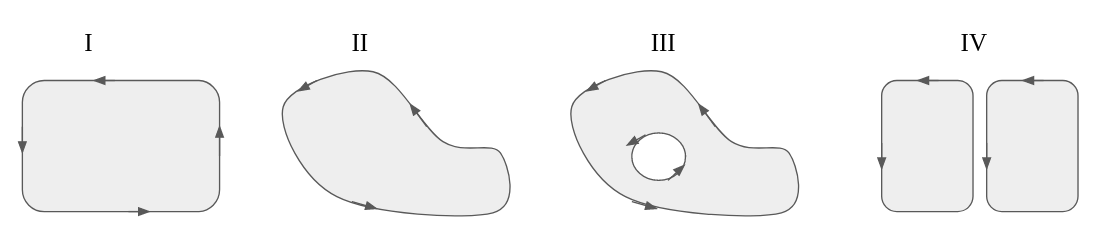
\includegraphics[width=10cm]{simply-connected.png}
	\end{center}

	\begin{center}
	Figure 1
\end{center}
	
	\par\noindent Given a field \(F=<P,Q>\) if R is a simply connected region with a boundary \(C\) oriented counterclockwise, and if \(P\) and \(Q\) have continuous first partial derivatives, then:
	
	\begin{flalign}
		\int_{C} P\;dx + Q\;dy = \int \int_{R}\frac{\partial Q}{\partial x} - \frac{\partial P}{\partial y}\;dA
	\end{flalign}

	\section{Alternative Line Integral Notation}
	
	\par\noindent Before we Expression (1) let's explain the notation used on the left, \(P\;dx + Q\;dy\). We start with the formulation for line integrals along a path \(C\):
	
	\begin{flalign*}
		\int_{C}F\;dr = \int_{a}^{b} F(r(t)) \cdot r'(t)\;dt
	\end{flalign*}

	\par\noindent Let's suppose \(F=<P,Q>\), then developing the dot product would get us:
	
	\begin{flalign*}
		\int_{a}^{b} <P,Q> \cdot <x'(t), y'(t)>\;dt
	\end{flalign*}
	
	\begin{flalign*}
		\int_{a}^{b} Px'(t) + Qy'(t)\;dt = \int_{a}^{b}Px'(t)\;dt + \int_{a}^{b}Qy'(t)\;dt =
		\int_{a}^{b}P\;\frac{dx}{dt}\;dt + 		\int_{a}^{b}Q\;\frac{dy}{dt}\;dt 
	\end{flalign*}

	\begin{flalign*}
		\int_{C} P\;dx + Q\;dy
	\end{flalign*}

	\par\noindent The use of this notation does not affect the calculation, but it does help with organization. Line integral and Green's Theorem problems are often presented in this format.
	
	\newpage
	
	\section{Deriving Green's Theorem}
	\par\noindent Given a field \(F=<P,Q>\) and our reformulated line integral \(\int_{C} P\;dx + Q\;dy\), we'll proceed to calculate the line integral along \(C\). We'll show the \(\int_{C}\;P\;dx\) on the left and \(\int_{C}\;Q\;dy\) on the right, combining the results at the end:
	\newline
	
	\begin{minipage}[t]{.5\linewidth}		
		\begin{center}
			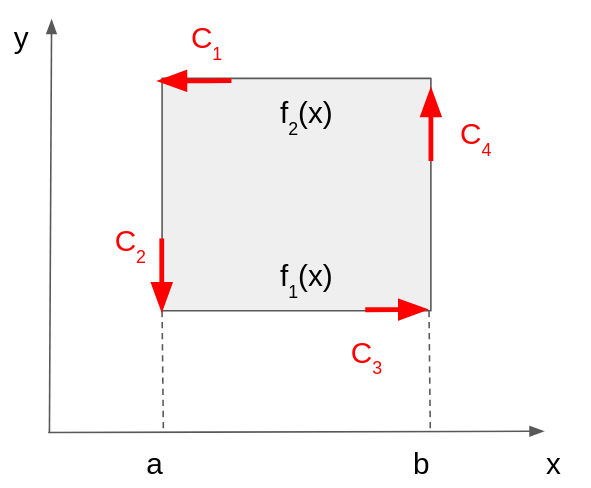
\includegraphics[width=5cm]{green-2.png}
		\end{center}
			\begin{center}
		Figure 2
	\end{center}
	\par\noindent In Figure 2 we've decomposed \(C\) into four paths \(C_1, C_2, C_3, C_4\). Since we are integrating with respect to \(x\) we can say that \(\int_{C_2}\;P\;dx = \int_{C_4}\;P\;dx = 0 \). For paths \(C_1\) and \(C_3\) the net line integral is:
	
	\begin{flalign*}
		-\int_{a}^{b}\;P(x,f_2(x))\;dx + \int_{a}^{b}\;P(x,f_1(x))\;dx
	\end{flalign*}

	\par\noindent The negative value refers to \(C_1\) based on its leftward direction. We can do some additional work with the result above:
	
	\begin{flalign*}
	-\int_{a}^{b}\;P(x,f_2(x))\;dx + \int_{a}^{b}\;P(x,f_1(x))\;dx \\
	= -\int_{a}^{b}\;P(x,f_2(x)) - \;P(x,f_1(x))\;dx 
\end{flalign*}

	\par\noindent By the Second Fundamental Theorem of Calculus:
	\begin{flalign*}
		-\int_{a}^{b}\;P(x,f_2(x)) - \;P(x,f_1(x))\;dx \\
		= -\int_{a}^{b}\;\int_{f_1(x)}^{f_2(x)}\;\frac{\partial P}{\partial y}\;dy\;dx \\
		= 
		- \int\;\int_{R} \frac{\partial P}{\partial y}\;dA
	\end{flalign*}
	
	
	\end{minipage}
\hspace{1cm}
	\begin{minipage}[t]{.5\linewidth}
		
		\begin{center}
			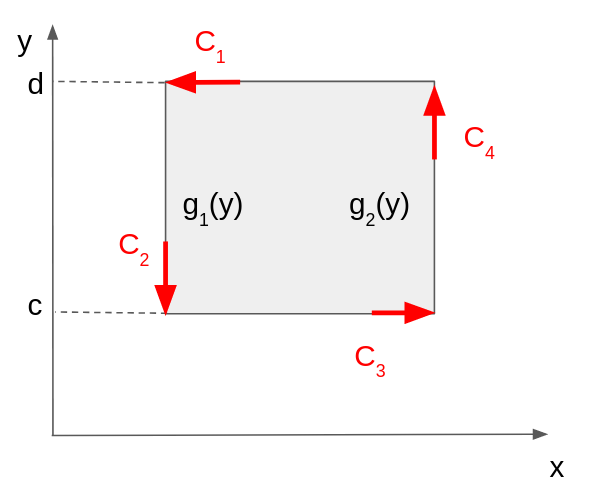
\includegraphics[width=5cm]{green-3.png}
		\end{center}
		
		\begin{center}
			Figure 3
		\end{center}
		
		\par\noindent We can repeat this process for \(\int Q\;dy\). Based on Figure 3's setup, we can say that \(\int_{C_1}Q\;dy = \int_{C_3}Q\;dy = 0 \). The net line integral we can come up with is:
		
		\begin{flalign*}
			\int_{c}^{d}\;Q(g_2(y),y)\;dy - Q(g_1(y), y)\;dy
		\end{flalign*}

		\par\noindent Applying the Second Fundamental Theorem of Calculus:
		
		\begin{flalign*}
			\int_{c}^{d}\;Q(g_2(y),y)\;dy - Q(g_1(y), y)\;dy \\
			= \int_{c}^{d}\;\int_{g_1(y)}^{g_2(y)}\;\frac{\partial Q}{\partial x}\;dx\;dy \\
			= \int \int_{R} \frac{\partial Q}{\partial x}\;dA
		\end{flalign*}
		
	\end{minipage}
\newline
\newline
		\par\noindent We bring both results together now:

\begin{flalign*}
	\int_{C}P\;dx + Q\;dy 
	= - \int\;\int_{R} \frac{\partial P}{\partial y}\;dA + \int \int_{R} \frac{\partial Q}{\partial x}\;dA 
	= \int \int_{R}\frac{\partial Q}{\partial x} - \frac{\partial P}{\partial y}\;dA 
\end{flalign*}
\section{Examples}
\framebox{
	\parbox{\linewidth}{
	\textbf{Ex.1} Calculate the line integral \(\int_{C}\;ye^x\;dx + 2e^x\;dy\). The path \(C\) is defined by a rectangle with points \((0,0), (3,0), (3,4), (0,4)\). Use both Green's Theorem and the traditional approach.
	\newline
	\par\noindent Source: Stewart, Calculus 8th Edition pg 1182
	\newline
	\par\noindent We will first use Green's Theorem:
	\begin{flalign*}
		\frac{\partial Q}{\partial x} = 2e^x \;\;\;\;\; \frac{\partial P}{\partial y} = e^x
	\end{flalign*}
	\par\noindent By the theorem we can evaluate the the following double integral:
	\begin{flalign*} \int_{0}^{4}\;\int_{0}^{3}\;2e^x - e^x\;dx\;dy
		=\int_{0}^{4}\;(2e^x - e^x) \Big|_0^{3}\;dy = \int_{0}^{4}\;e^3-1\;dy = (e^3-1)y\Big|_0^{4} =
		4(e^3-1)
	\end{flalign*}
	\par\noindent We arrived at the answer with relative ease using Green's Theorem. We will now attempt the long way. Let's define the path going along the bottom edge as \(C_1\), the right edge \(C_2\), the top edge \(C_3\) and the left edge \(C_4\).
	\newline
	\par\noindent \(C_1\): 
	\par\noindent We can start by defining \(r(t) = <t,0>\), which makes \(r'(t)=<1,0>\). We can now say that \(F(r(t)) = <0,2e^t>\). Since \(F(r(t)) \cdot r'(t)\) = 0, then the line integral along \(C_1\) is 0.
	\newline
	\par\noindent \(C_2\): 
	\par\noindent Here we can say that \(r(t) = <3,t>\) so \(r'(t) = <0,1>\). So then \(F(r(t)) = <te^3,2e^3>\), and \(F(r(t)) \cdot r'(t) = 2e^3\). We can now compute the following integral:
	\begin{flalign*}
		\int_{0}^{4}\;2e^3\;dt =  8e^3
	\end{flalign*}
	\par\noindent \(C_3\): 
	\par\noindent Starting the same way we have \(r(t) = <-t,4>\) and \(r'(t) = <1,0>\). So then \(F(r(t)) = <4e^{t}, 2e^t>\), and \(F(r(t)) \cdot r'(t) = -4e^{-t}\). We are left with the following integral:
	\begin{flalign*}
		\int_{0}^{3}\;-4e^{t}\;dt = 4e^{t} \Big|_0^{4} = 4e^{3} - 4
	\end{flalign*}
	\par\noindent \(C_4\): 
	\par\noindent For the last segment of the path, we have \(r(t)=<0,t>\), \(r'(t) = <0,1>\), \(F(r(t)) = <t,2>\), and \(F(r(t))\cdot r'(t) = 2\). We just have to complete the following integral:
	\begin{flalign*}
		\int_{0}^{4}\;2\;dt = 8
	\end{flalign*}
	\par\noindent We can conclude the process by adding the line integral for each of the four paths. We will give the result for \(C_3\) and \(C_4\) as negatives since they move left and down respectively: 
	\begin{flalign*}
		8e^3 - 8 - (4e^3 - 4) = 4(e^3-1).
	\end{flalign*}
}}
\newpage
\framebox{
	\parbox{\linewidth}{
		
		
		\par\noindent \textbf{Ex.2} Evaluate \(\int_{C} \cos y \; dx + (xy-x\sin y)\; dy\) using Green's Theorem. C is the boundary of the area formed between \(y=\sqrt{x}\) and \(y=x\).
		\newline
		\par\noindent Source: Larson, Calculus 6th Edition, pg 1061
		\newline
		\begin{flalign*}
			\frac{\partial Q}{\partial x} = y-\sin y \;\;\;\; \frac{\partial P}{\partial y} = - \sin y
		\end{flalign*}
		\par\noindent Here is a graph showing the bounds of integration:
			\begin{center}
			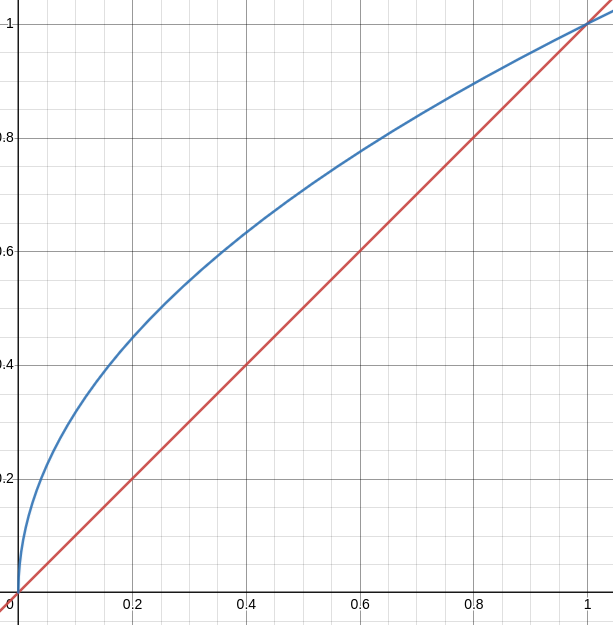
\includegraphics[width=3cm]{green-4.png}
		\end{center}
		\begin{center}
			Figure 4
		\end{center}
	
		\begin{flalign*}
			\int_{0}^{1}\;\int_{x}^{\sqrt{x}}\; y - \sin y - (-\sin y) \; dy \; dx = \int_{0}^{1}\;\frac{y^2}{2} \Big|_x^{ \sqrt{x}}\;dx \\
			=\frac{1}{2}\int_{0}^{1} x - x^2 \;dx = \frac{1}{2}(\frac{x^2}{2} - \frac{x^3}{3}) \Big|_0^{1} \\= \frac{1}{12}
		\end{flalign*}
	

\
}}
\newline
\newline

\framebox{
	\parbox{\linewidth}{
\textbf{Ex. 3} Evaluate \(\int_{C}\;y^3\;dx - x^3\;dy\) where \(C\) is the edge of a circle with radius 2.
\newline
		\par\noindent Source: Larson, Calculus 6th Edition, pg 1061
		\newline
		\begin{flalign*}
			\frac{\partial Q}{\partial x} = -3x^2 \;\;\;\; \frac{\partial P}{\partial y} = 3y^2
	\end{flalign*}	
		\par\noindent Applying the theorem, we get:
		
		\begin{flalign*}
			\int_{a}^{b}\;\int_{c}^{d}\;-3x^2 - 3y^2\;dy\;dx
		\end{flalign*}
		\par\noindent The best way to proceed is to change over to polar coordinates, so we have:
		\begin{flalign*}
-3 \int_{0}^{2\pi}\;\int_{0}^{2}\;(r^2)r\;dr\;d\theta = -3 \int_{0}^{2\pi} = -3 \int_{0}^{2\pi}\;\frac{r^4}{4} \Big|_0^{2}\;d\theta \\
-3 \int_{0}^{2\pi}\;4\;d\theta = -3(4\theta) \Big|_0^{2\pi} \\= -24\pi
		\end{flalign*}
		
}}
	
\end{document}